\chapter{Deployment}

The deployment of the system is done on a Kubernetes cluster hosted on Google Cloud. The end result deployment architecture is almost identical to the established architecture in the design phase. Nothing of particular importance had to change in order to deploy the established design on a Kubernetes cluster, though some very minor changes had to be done. The deployment architecture shown below, is of the Odin configuration, which uses the Peer-to-peer WebRTC solution. 

\begin{figure}[ht]
    \centering
    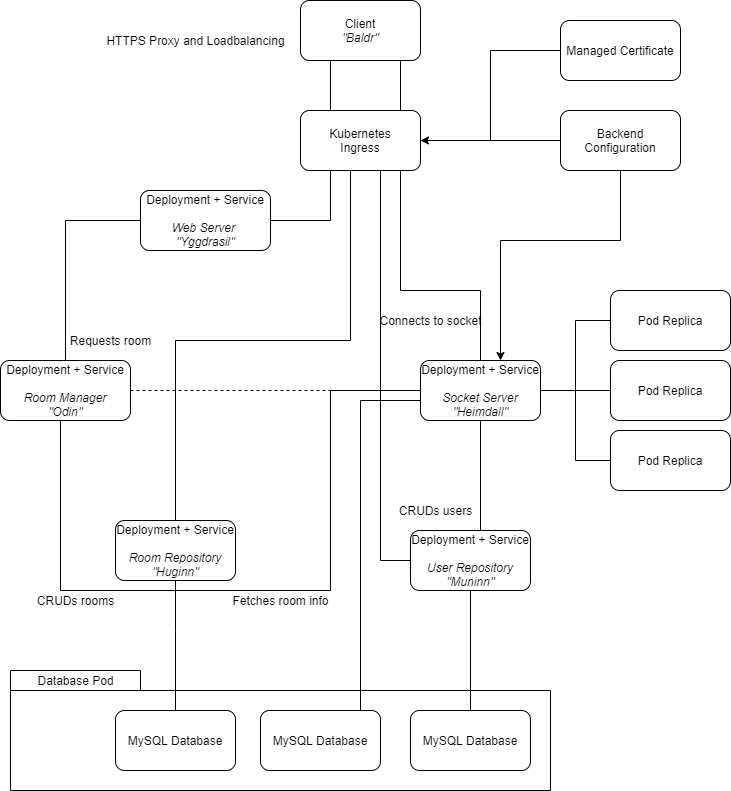
\includegraphics[width=\textwidth]{Pictures/Odin Kubernetes Deployment (2).png}
    \caption{A diagram showing the Design architecture described with the deployments and services in the Kubernetes cluster deployment }
    \label{fig:gantt}
\end{figure}

All configuration files used can be found under this link \cite{kubernetes-settings}



\section{Ingress}

The system back end is behind an Ingress load-balancer that handles the external access to the system. The Ingress contains a number of paths that lead to specified services in the Kubernetes namespace. When these paths are connected to, either via an API or through a web browser, the Ingress leads to the service defined under said path. 

To expose the Ingress an external IP is created and bound to the ingress in order to gain access remotely. This is done using Google Cloud. Through Google Cloud, a static external IP is created and attached to the Ingress. Through that IP it is now possible to access the services connected to the Ingress Load-Balancer. 
In addition to external access, a certificate is added to the Ingress in order to gain TLS on the connections. This is done through a ManagedCertificate configuration applied to the Kubernetes cluster. Googles Ingress Controller automatically talks with Googles Certificate Providers, so when applied, the certificate provision is started automatically. The only requirement is to connect a domain name to the external IP. This was done using Cloudflare.

After all these configurations, CoffeeBreak is publicly available on a self provided domain, with HTTPS connection.

\section{Shared Components in the Twin Designs}

The shared system components consists of "Yggdrasil", the web server that serves the website client. The room repository, "Huginn", that handles room CRUD operations with the client and room database creation and fetching. The user repository, "Muginn", that handles the user CRUD Operations with the client and user database creation and fetching. Lastly, the room manager, "Odin" which handles room creation. 

The above mentioned services all are configured to be a Deployment that has a single Pod, and a Service on top. The Service exposes the pod IP and communication in order for the Ingress to publicly expose them to the internet. The Deployment configuration contains the name of the application, what port the container should open, the image of the container and a number of environmental variables. These environmental variables contain the different information required to know, in order to connect to the other services in the Kubernetes cluster. 

The Service configuration contains the label of which Deployment it should be connected to, target port of said deployment, and the port it should forward the target port to. 

Setting it up like this makes it easy to give access to each Service externally through the Ingress or creating more replicas if required through the Deployment configuration. In this case, since most of the traffic goes through the Socket Server “Heimdall”, the Deployments does not have any replicas, other than "Yggdrasil".

\section{The Socket Server}

The socket server “Heimdall” is the heart of the system, serving both the room and the signalling socket server. The room socket server handles user positions, chat messaging, and more in each room, while the signalling server handles the WebRTC signalling between all users. This causes it to potentially receive a large amount of traffic depending on the amount of users. To counteract this a deployment solution had to be found in order to prevent a bottleneck in the system. The solution found is to have multiple replicas of the Socket Server service. This would split the incoming traffic between the replicas. However with socket servers, if two users connect to the same room, but different replicas, they would receive any messages sent to each other. A system needs to be set in place in order to update all socket server replicas. 

This is done with Redis. Redis handles the messages sent to the separate replicas of the socket server and publishes them to all the others replicas subscribed to the redis implementation. 

The Socket Server “Heimdall” has three replicas by default. A redis master-slave system is created in order to keep track of the different socket server replicas and update them in order for users connected to different replicas, still be able to communicate with each other. Below is an illustration of this configuration. 
\begin{figure}[ht]
    \centering
    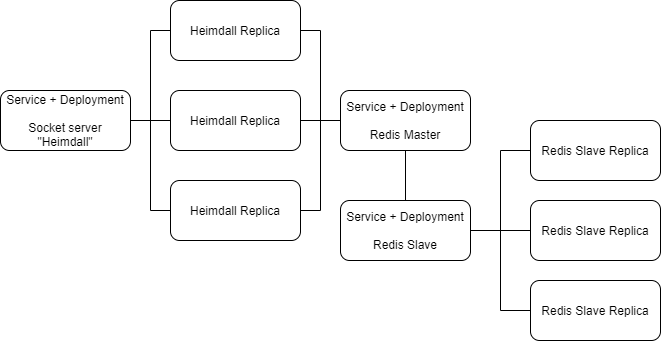
\includegraphics[width=\textwidth]{Pictures/Redis configuration.png}
    \caption{A diagram showing the relationship between the socket server replicas and the redis implementation}
    \label{fig:gantt}
\end{figure}
In order for this configuration to work as intended it is important to implement a sticky session between the user and the connected Socket Server replica. This sticky session ensures that the user is connected to the same replica throughout the socket connection. A BackendConfig is applied to the cluster and inserted as an annotation in the Ingress configuration and the Heimdall service configuration file. 

\section{Pod Auto scaling}

The web server, Yggdrasil, and the Socket Server, Heimdall, also has a horizontal pod autoscaler implemented. This is to automatically increase scalability in case of the initial three replicas is not enough to cope with the current load. A Metrics Server is applied to the cluster in order to monitor resource usage across pods on the cluster. Using this information, the autoscalers connected to the deployments create or delete replicas in line with workload.

\section{The Database}

The database is a simple pod implementation of a stock MySQL database. The IP of the pod is entered as an environmental variable in order for the services to connect. 

\section{Conclusion}

Deployment of the system to a Kubernetes Cluster makes it simple to create scalable modifications to an existing architecture that seems rigid in nature. Using the different aspects of Kubernetes in general and Google Clouds’ Kubernetes Engine, it is possible to establish a fully fledged system that is scalable in order to reach the goals established at the start of the project. 
